\documentclass[main.tex]{subfiles}

\begin{document}

\subsection{Terzo esercizio}
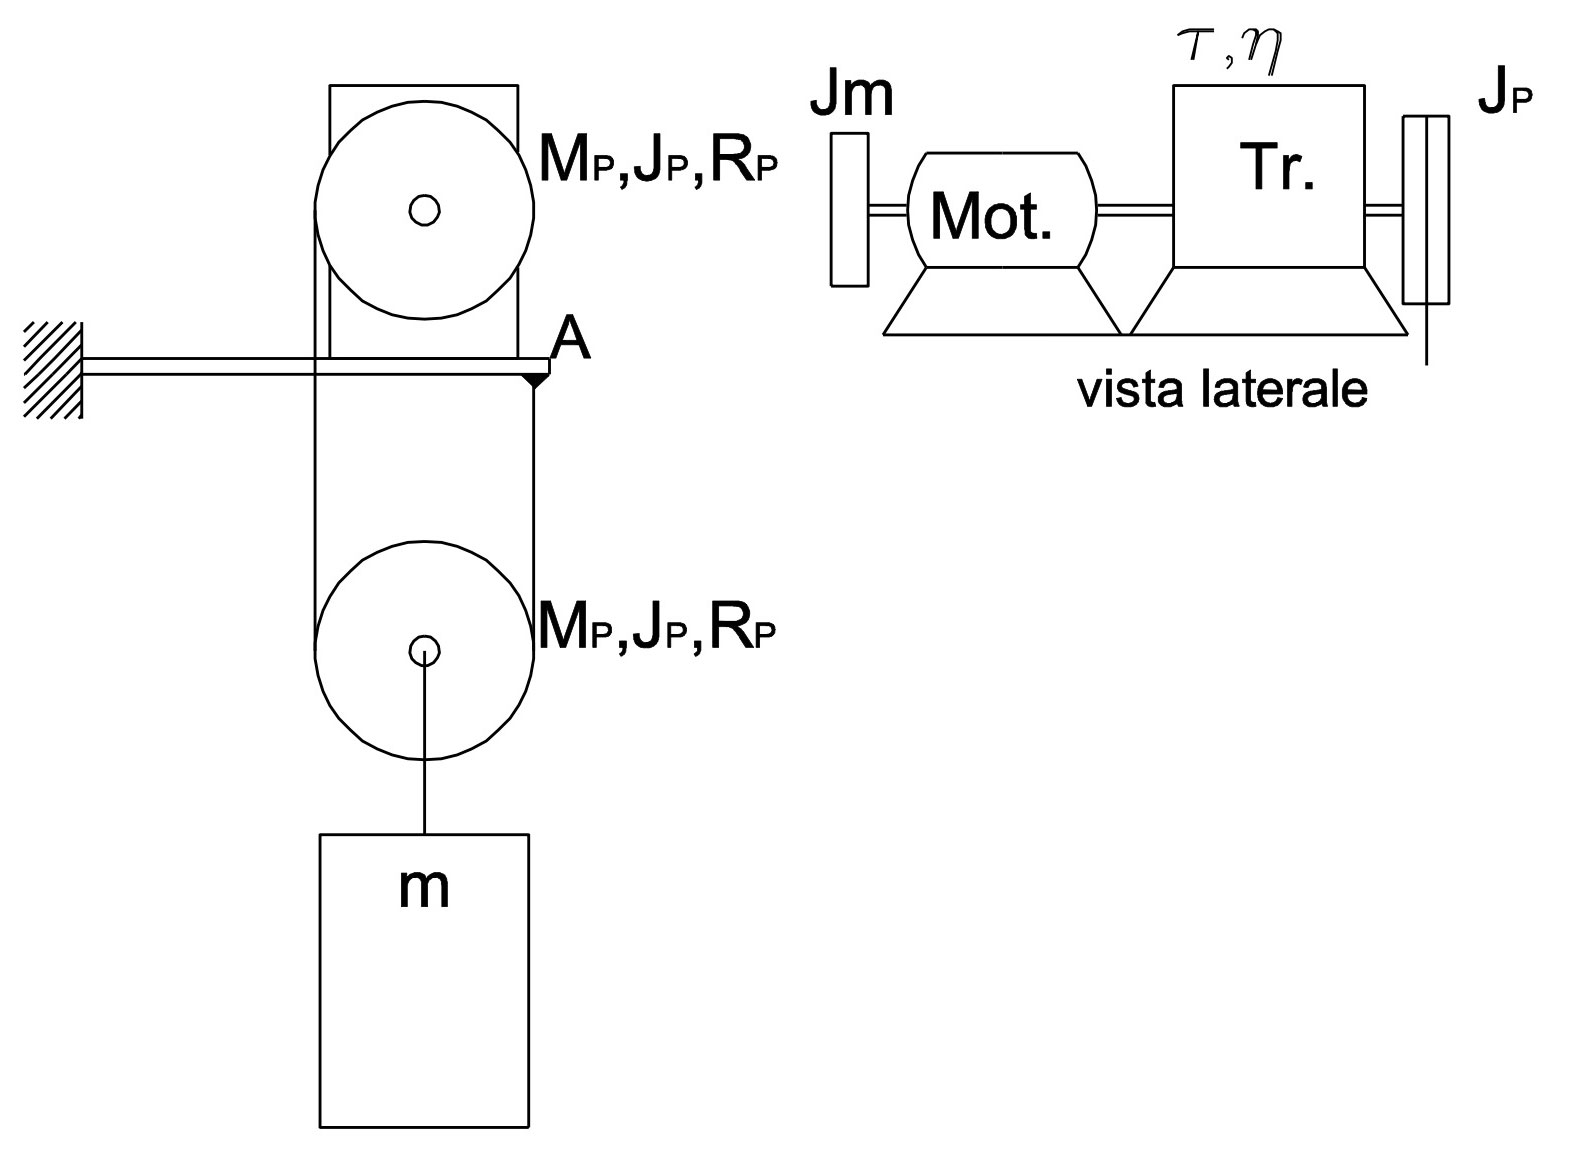
\includegraphics[width=\textwidth]{2015-0109-3.jpg}

\[
	m =120\,Kg \quad
	J_P = 0.2\,Kgm^2 \quad
	R_P = 0.15\,m \quad
	M_P = 20\, Kg \quad
	J_m = 0.1\,Kgm^2 \quad
\]
\[
	\tau = 1/50 \quad
	\mu_D = 0.9 \quad
	\mu_R = 0.7 \quad
	C_{m0} = 12\,Nm \quad
	A = 0.02\,Nm/(rad/s)
\]

\[
	C_m = C_{m0} - A\omega_m
\]

Il sistema rappresentato in figura, posto nel piano verticale, rappresenta un impianto di sollevamento. Un motore, avente momento d'inerzia $J_m$ e curva caratteristica della coppia motrice assegnata, è collegato per mezzo di una trasmissione (rapporto di trasmissione $\tau$, rendimento in moto diretto $\mu_D$, rendimento in moto retrogrado $\mu_R$) ad una puleggia avente massa $M_p$, momento d'inerzia $J_p$ e raggio $R_p$. La puleggia, a sua volta, movimenta una seconda puleggia mobile identica alla prima tramite una fune inestensibile che si avvolge sulla prima puleggia ed è collegata a terra nell’estremo in A. Al centro della seconda puleggia è, infine, collegato un carico avente massa $m$.

Si chiede di calcolare:

\begin{enumerate}
\item La coppia motrice e la potenza erogate dal motore nel caso di sollevamento a velocità costante del carico $m$.
\item La coppia motrice nel caso di moto in discesa del carico $m$ con decelerazione $a_m$ nota pari a $0.05\,m/s^2$.
\end{enumerate}

\clearpage

\subsection{Soluzione terzo esercizio}

\subsubsection{Osservazioni}

\begin{enumerate}
\item La velocità nel primo punto è costante. Questo implica che ci troviamo in \textbf{condizioni di regime}.
\end{enumerate}

\subsubsection{Primo punto}

\paragraph{Calcolo della potenza motrice}

\[
	W_m = C_m\omega_m
\]

\paragraph{Calcolo della potenza resistente}
Per calcolare la potenza resistente $W_r$ considero tutte le forze agenti sul sistema: forze peso, attriti (statici, dinamici e volventi) e forze esterne in generale, che vengano applicate ad una massa in moto.

\begin{enumerate}
\item La forza peso agente sulla massa della puleggia superiore è contro bilanciata da una forza normale. Essa agisce sul baricentro della puleggia, che è implicitamente indicato come coincidente con il centro della stessa, per cui non vi è nè moto traslatorio nè rotatorio.
\item La forza peso agente sulla massa della puleggia inferiore, a differenza di quella superiore, contribuisce alla potenza resistente poiché il centro della massa si muove verticalmente. Siamo nel caso di un sollevamento, per cui la forza peso forma un angolo di $\pi$ con la velocità.
\item Discorso analogo può essere fatto per la massa $m$, che può essere sommata alla massa $M_P$ per quanto riguarda il contributo della forza peso.
\end{enumerate}

\[
	W_r = \vec{F}_{g_{m+M_P}}\bullet\vec{v}
\]

Risolvo il prodotto scalare:

\[
	W_r = F_{g_{m+M_P}}v\cos\pi = - F_{g_{m+M_P}}v
\]

Definisco la forza peso:

\[
	F_{g_{m+M_P}} = (M_P + m)g
\]

Determino il legame cinematico della velocità, considerato come CIR il punto della corda aderente alla puleggia inferiore:

\[
	v_{sollevamento tangente} = R_P\omega_P = R_P\tau\omega_m
\]

\[
	v = v_{sollevamento} = \dfrac{R_P}{2R_P}v_{sollevamento tangente} = \dfrac{1}{2}v_{sollevamento tangente} = \dfrac{1}{2}R_P\tau\omega_m
\]

Sostituendo entrambe le formule così ottenute, ottengo:

\[
	W_r = -\dfrac{1}{2}(M_P + m)gR_P\tau\omega_m
\]

\paragraph{Indentificazione del tipo di moto} Per identificare il tipo di moto con cui il sistema di sollevamento si muove, siccome siamo in condizioni di regime, è sufficiente controllare il segno della potenza resistente:

\[
	W_r > 0
\]

Se la disequazione risultasse vera, allora siamo in condizioni di \textbf{moto retrogrado}, altrimenti \textbf{diretto}.

\[
	 -\dfrac{1}{2}(M_P + m)gR_P\tau\omega_m > 0
\]

Nessuno dei termini ha segno negativo, per cui l'equazione è certamente falsa.

Siamo quindi in condizioni di \textbf{moto diretto}.

\paragraph{Calcolo della potenza perduta} Essendo in condizioni di moto diretto e regime, utilizzo la formula corrispondente:

\[
	W_p = -(1-\mu_D)W_m
\]

\paragraph{Bilancio delle potenze} Usando la formula del bilancio delle potenze calcolo il valore della velocità angolare $\omega_m$:

\[
	W_m + W_r + W_p = 0
\]

\[
	W_m + W_r - (1-\mu_D)W_m = 0
\]

\[
	W_r + \mu_DW_m = 0
\]

\[
	\mu_DC_m\omega_m -\dfrac{1}{2}(M_P + m)gR_P\tau\omega_m= 0
\]

\[
	\mu_DC_m -\dfrac{1}{2}(M_P + m)gR_P\tau = 0
\]

Sostituisco con la formula fornita ed ottengo:

\[
	\mu_D(C_{m0}-A\omega_m) -\dfrac{1}{2}(M_P + m)gR_P\tau = 0
\]

\[
	\mu_DA\omega_m = \mu_DC_{m0} - \dfrac{1}{2}(M_P + m)gR_P\tau
\]

\[
	\omega_m = \dfrac{\mu_DC_{m0} - \dfrac{1}{2}(M_P + m)gR_P\tau}{\mu_DA}
\]

Sostituisco numericamente ed ottengo:

\[
	\omega_m = 485.55\,rad/s
\]

Sostituisco il valore ottenuto nella formula della coppia motrice ed ottengo:

\[
	C_m = 2.289\,Nm
\]

Sostituisco nella formula della potenza motrice ed ottengo:

\[
	W_m = 1111.4\,W
\]

\subsubsection{Secondo punto}
Esiste una decelerazione $a_m$, per cui certamente non siamo più in condizioni di regime ma di \textbf{transitorio}.

La posizione del CIR della puleggia inferiore cambia poiché siamo in caso di moto in discesa. Esso si trova nel punto di tangenza sinistro, tra corda e puleggia.

\paragraph{Identifico legame cinematico per accelerazione} Per utilizzare il dato fornito per l'accelerazione $a_m$, cerco un legame cinematico tra essa ed $\dot{\omega}_m$:

\begin{center}
\framebox[4in]{
\begin{minipage}[t]{3.5in}
{\Large{\danger}} \textbf{N.B.}
L'accelerazione data nel testo ha segno negativo rispetto alla direzione del moto, essendo una decelerazione.
\end{minipage}}
\end{center}

\[
	a_m = \dfrac{1}{2}R_P\dot{\omega}_m\tau \Longrightarrow \dot{\omega}_m = \dfrac{2a_m}{R_P\tau} = -33.3\,rad/s^2
\]

\paragraph{Calcolo energia cinetica totale} Per calcolare l'energia cinetica totale considero i momenti di inerzia baricentrici di tutti i corpi rotanti e le masse di tutti gli oggetti in moto traslatorio.

Identificando il legame cinematico della velocità della massa $m$, $v$, ottengo l'energia cinetica:

\[
	v = \dfrac{1}{2}R_P\omega_m\tau
\]

\begin{align*}
	E_c &= \dfrac{1}{2}J_m\omega_m^2 + J_P(\omega_m\tau)^2 + \dfrac{1}{2}(M_P + m)v^2 \\
	&=  \dfrac{1}{2}J_m\omega_m^2 + J_P(\omega_m\tau)^2 + \dfrac{1}{2}(M_P + m)(\dfrac{1}{2}R_P\omega_m\tau)^2
\end{align*}

Raccolgo i coefficienti in comume:

\[
	 E_c = \omega_m^2(\dfrac{1}{2}J_m + \tau^2(J_P + \dfrac{1}{8}(M_P + m)R_P^2))
\]

Derivo l'espressione dell'energia cinetica ed ottengo:

\[
	 \dfrac{dE_c}{dt} = \omega_m\dot{\omega}_m(J_m + \tau^2(2J_P + \dfrac{1}{4}(M_P + m)R_P^2))
\]

\paragraph{Identifico il tipo del moto} Essendo in condizioni di transitorio, va considerata anche l'energia cinetica nella disequazione. Se questa risulta vera, siamo in condizioni di \textbf{moto retrogrado}, \textbf{diretto} altrimenti.

\begin{center}
\framebox[4in]{
\begin{minipage}[t]{3.5in}
{\Large{\danger}} \textbf{N.B.}
La direzione del moto è cambiata, il vettore velocità ora è concorde con la forza peso e quindi cambia il segno del prodotto scalare con essa. La potenza resistente, quindi, cambia di segno.
\end{minipage}}
\end{center}

\[
	W_r = \dfrac{1}{2}(M_P + m)gR_P\tau\omega_m
\]

\[
	W_r - \dfrac{dE_{c_r}}{dt} > 0
\]

\[
	\dfrac{1}{2}(M_P + m)gR_P\tau\omega_m - \omega_m\dot{\omega}_m(\tau^2(2J_P + \dfrac{1}{4}(M_P + m)R_P^2)) > 0
\]

\[
	\dfrac{1}{2}(M_P + m)gR_P\tau - \dot{\omega}_m(\tau^2(2J_P + \dfrac{1}{4}(M_P + m)R_P^2)) > 0
\]

\[
	2.07 > 0
\]

L'equazione è vera, per cui il moto è \textbf{retrogrado}.

\paragraph{Calcolo la potenza perduta} Siamo in condizioni di moto retrogrado e transitorio, per cui la formula della potenza perduta da utilizzare è la seguente:

\begin{align*}
	W_p &= -(1-\mu_r)(W_r - \dfrac{dE_{c_r}}{dt}) \\
	&= -(1-\mu_r)(\dfrac{1}{2}(M_P + m)gR_P\tau\omega_m - \omega_m\dot{\omega}_m(\tau^2(2J_P + \dfrac{1}{4}(M_P + m)R_P^2)))
\end{align*}

\paragraph{Bilancio delle potenze} Utilizzo il bilancio delle potenze e risolvo per $C_m$:

\begin{equation}
	W_m + W_r + W_p = \dfrac{dE_c}{dt}
\end{equation}

\begin{equation}
	W_m + W_r -(1-\mu_r)(W_r - \dfrac{dE_{c_r}}{dt}) = \dfrac{dE_c}{dt}
\end{equation}

Semplifico la potenza resistente:

\begin{equation}
	W_m + \mu_r(W_r - \dfrac{dE_{c_r}}{dt}) = \dfrac{dE_c}{dt}
\end{equation}

Separo le componenti dell'energia cinetica:

\begin{equation}
	W_m + \mu_r(W_r - \dfrac{dE_{c_r}}{dt}) = \dfrac{dE_{c_r}}{dt} + \dfrac{dE_{c_m}}{dt}
\end{equation}

Sposto a secondo membro l'energia cinetica:

\begin{equation}
	W_m + \mu_rW_r = \dfrac{dE_{c_r}}{dt} + \dfrac{dE_{c_m}}{dt} + \mu_r\dfrac{dE_{c_r}}{dt}
\end{equation}

Raccolgo a secondo membro:

\begin{equation}
	W_m + \mu_rW_r = \dfrac{dE_{c_r}}{dt} + \dfrac{dE_{c_r}}{dt}(1+\mu_r)
\end{equation}

Sostituisco i termini con le relative espressioni:

\begin{equation}
	C_m\omega_m + \mu_r\dfrac{1}{2}(M_P + m)gR_P\tau\omega_m =  \omega_m\dot{\omega}_mJ_m +\omega_m\dot{\omega}_m(\tau^2(2J_P + \dfrac{1}{4}(M_P + m)R_P^2))(1+\mu_r)
\end{equation}

Semplifico la velocità angolare $\omega_m$:

\begin{equation}
	C_m + \mu_r\dfrac{1}{2}(M_P + m)gR_P\tau =  \dot{\omega}_mJ_m + \dot{\omega}_m(\tau^2(2J_P + \dfrac{1}{4}(M_P + m)R_P^2))(1+\mu_r)
\end{equation}

Raccolgo a secondo membro i coefficienti di $\dot{\omega}_m$:

\begin{equation}
	C_m + \mu_r\dfrac{1}{2}(M_P + m)gR_P\tau =  \dot{\omega}_m(Jm + \tau^2(2J_P + \dfrac{1}{4}(M_P + m)R_P^2)(1+\mu_r))
\end{equation}

Risolvo per $C_m$:

\begin{equation}
	C_m =  \dot{\omega}_m(Jm + \tau^2(2J_P + \dfrac{1}{4}(M_P + m)R_P^2)(1+\mu_r)) - \mu_r\dfrac{1}{2}(M_P + m)gR_P\tau
\end{equation}

Sostituisco numericamente ed ottengo:

\[
	C_m = -4.76\,Nm
\]

\end{document}